\Def Диаметром $S \subset \R^2, |S| < \infty$ называют такую пару $a, b \in S$, на которой достигается максимум $||a - b||$.

\Task Надо найти диаметр по евклидовой метрике.

\Statement Концами диаметра являются две вершины выпуклой оболочки $S$.

\Proof Пусть $AB$ — диаметр $S$, при этом $B$ — не вершина выпуклой оболочки. Рассмотрим луч $AB$ и пересечем его с $conv(S)$ в точке $C$. Тогда $|AC| \Ge |AB|$. Теперь пусть $PQ$ — сторона $conv(S)$, по которой луч $AB$ пересек $conv(S)$. Очевидно, $\max(|AP|, |AQ|) > |AC| \Ge |AB|$, откуда $AB$ не диаметр.

\begin{figure}[h]
    \centering
    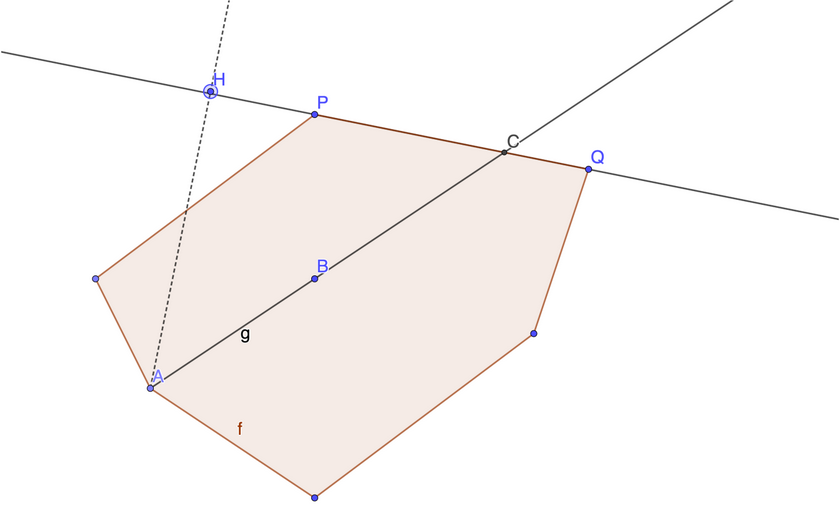
\includegraphics[scale = 0.8]{pix/pair_far1.png}
\end{figure}

\Task Дан выпуклый многоугольник $P_0, \dots, P_{n-1}$. Найдите пару $i, j \in \overline{(0, n - 1)}$, что $||P_i - P_j ||$ по евклидовой метрике максимально.

\vspace{\baselineskip}

\Def Прямая $L$ опорная для выпуклого многоугольника $P_0, \dots, P_{n-1}$, если вся внутренность лежит по одну полуплоскость относительно $L$ и $\exists i : P_i \in L$.

\Statement Пусть $L_1$ и $L_2$ — две параллельные опорные прямые фигуры Ф, расстояние между которыми имеет максимальное значение. $A_1$ и $A_2$ — граничные точки фигуры Ф, принадлежащие соответственно прямым $L_1$ и $L_2$. Тогда отрезок $A_1A_2$ перпендикулярен обеим прямым $L_1$ и $L_2$.

\Proof Предположим, что это не так. Тогда расстояние между прямыми $L_1$ и $L_2$ было бы меньше, чем отрезок $A_1A_2$, и тем более меньше, чем расстояние между двумя опорными прямыми $L^{'}_{1}$ и $L^{'}_{2}$ фигуры Ф, перпендикулярными к отрезку $A_1A_2$, что противоречит условию.


(рисунок ниже)

\begin{figure}[h]
    \centering
    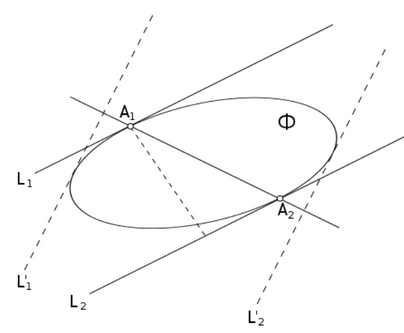
\includegraphics[scale = 1]{pix/pair_far3.png}
\end{figure}

\vspace{\baselineskip}

\Th\textit{(о диаметре)} Диаметр выпуклого многоугольника равен максимальному расстоянию между параллельными опорными прямыми.

\Proof Пусть $L_1$ и $L_2$ — параллельные опорные прямые, на которых достигается максимальное расстояние $d$. Тогда $A_1A_2 \perp L_i$. Допустим, что есть две точки $B_1, B_2$, расстояние между которыми больше. Тогда рассмотрим ортогональные $B_1B_2$ опорные прямые $L^{'}_{1}, L^{'}_{2}$. $|B_1B_2| \Le dist(L^{'}_{1}, L^{'}_{2}) \Le d$.

\vspace{\baselineskip}

\Alg
\begin{enumerate}
    \item Построим $P = conv(S)$.
    \item Пусть $A_1 = P_0$, тогда $A_2$ — максимально удаленная от $A_1$ точка $P$.
    \item Заведем два указателя на $A_1$ и $A_2$ и будем идти против часовой стрелки. Двигается тот указатель, который указывает на угол меньший до проворота.
\end{enumerate}

\begin{figure}[h]
    \centering
    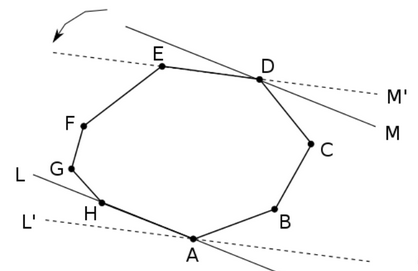
\includegraphics[scale = 1]{pix/pair_far2.png}
\end{figure}
\pagebreak